% ju 31-Jul-20
\documentclass[a4paper,12pt]{scrartcl}
% letztes Update: 1-Jun-20

% Eingabe der Metadaten

%-------Daten des Autors--------------------------
\newcommand{\autor}{Jan Unger}
\newcommand{\ort}{Wuppertal}
\newcommand{\website}{https://bw-ju.de/}

%-------Titel und Untertitel-----------------------
\newcommand{\titel}{Markdown -- Latex}% THEMA 
\newcommand{\untertitel}{}% keinen Untertitel 
\newcommand{\typ}{Projekt}

%-------Datum: Jahr/Monat/Tag ---------------------
\newcommand{\version}{\today}% DATUM:  \date{2020/06/30}  o. \today

%-deutsche Schlagwoerter(bitte getrennt durch Kommata auflisten)
\newcommand{\schlagwoerter}{PDF, Latex, Markdown, Pandoc, Git, Texlive}



%% anpassen
\usepackage{praeambel-artikel}% Pakete
% Literatur laden
\bibliography{content/literatur}      %% anpassen
\bibliography{content/literatur-kfz}  %% anpassen
\bibliography{content/literatur-sport}%% anpassen
%% anpassen
\title{Spickzettel-Markdown}
\author{\autor}
\date{\today}
%\date{2020/08/01}%% anpassen
%\date{1-Aug-20}
%
\begin{document}
	%% anpassen
	%\maketitle
	%\tableofcontents  
	%\listoffigures 
	%\listoftables 
	%\lstlistoflistings

	%% anpassen	
	%\begin{abstract}
	%	Zusammenfassung
	%\end{abstract}

		%% anpassen
		%-------------------------------------------------
		%
			% letztes Update: 01-Aug-20
\section{Quellen}\label{quellen}

Quelle: ~\textcite{monk:2016:action}

Quelle: ~\textcite{homofaciens:2018:projekt}

Quelle: ~\textcite{kofler:2018:hacking}

\section{Listen}\label{listen}

\textbf{ungeordnete Liste}

\begin{itemize}
\item
  a
\item
  b

  \begin{itemize}
  \item
    bb
  \end{itemize}
\item
  c
\end{itemize}

\textbf{Sortierte Liste}

\begin{enumerate}
\item
  eins
\item
  zwei
\item
  drei
\end{enumerate}

\textbf{Sortierte Liste}

\begin{enumerate}
\def\labelenumi{\alph{enumi})}
\item
  a
\item
  b
\item
  c
\end{enumerate}

\section{Anführungszeichen}\label{anfuehrungszeichen}

>>Anführungszeichen<<

\section{Bilder -- Abbildungen}\label{bilder-abbildungen}

Logo vgl.~(\autoref{fig:Logo}).

\begin{figure}[!hb]% hier: !hb
\centering

\includegraphics[width=0.6\textwidth]{images/logo.eps}
\caption{Logo}
\label{fig:Logo}%% anpassen
\end{figure}

Abbildung-Bsp vgl.~(\autoref{fig:Abbildung-Bsp}).

\begin{figure}[!hb]% hier: !hb
\centering
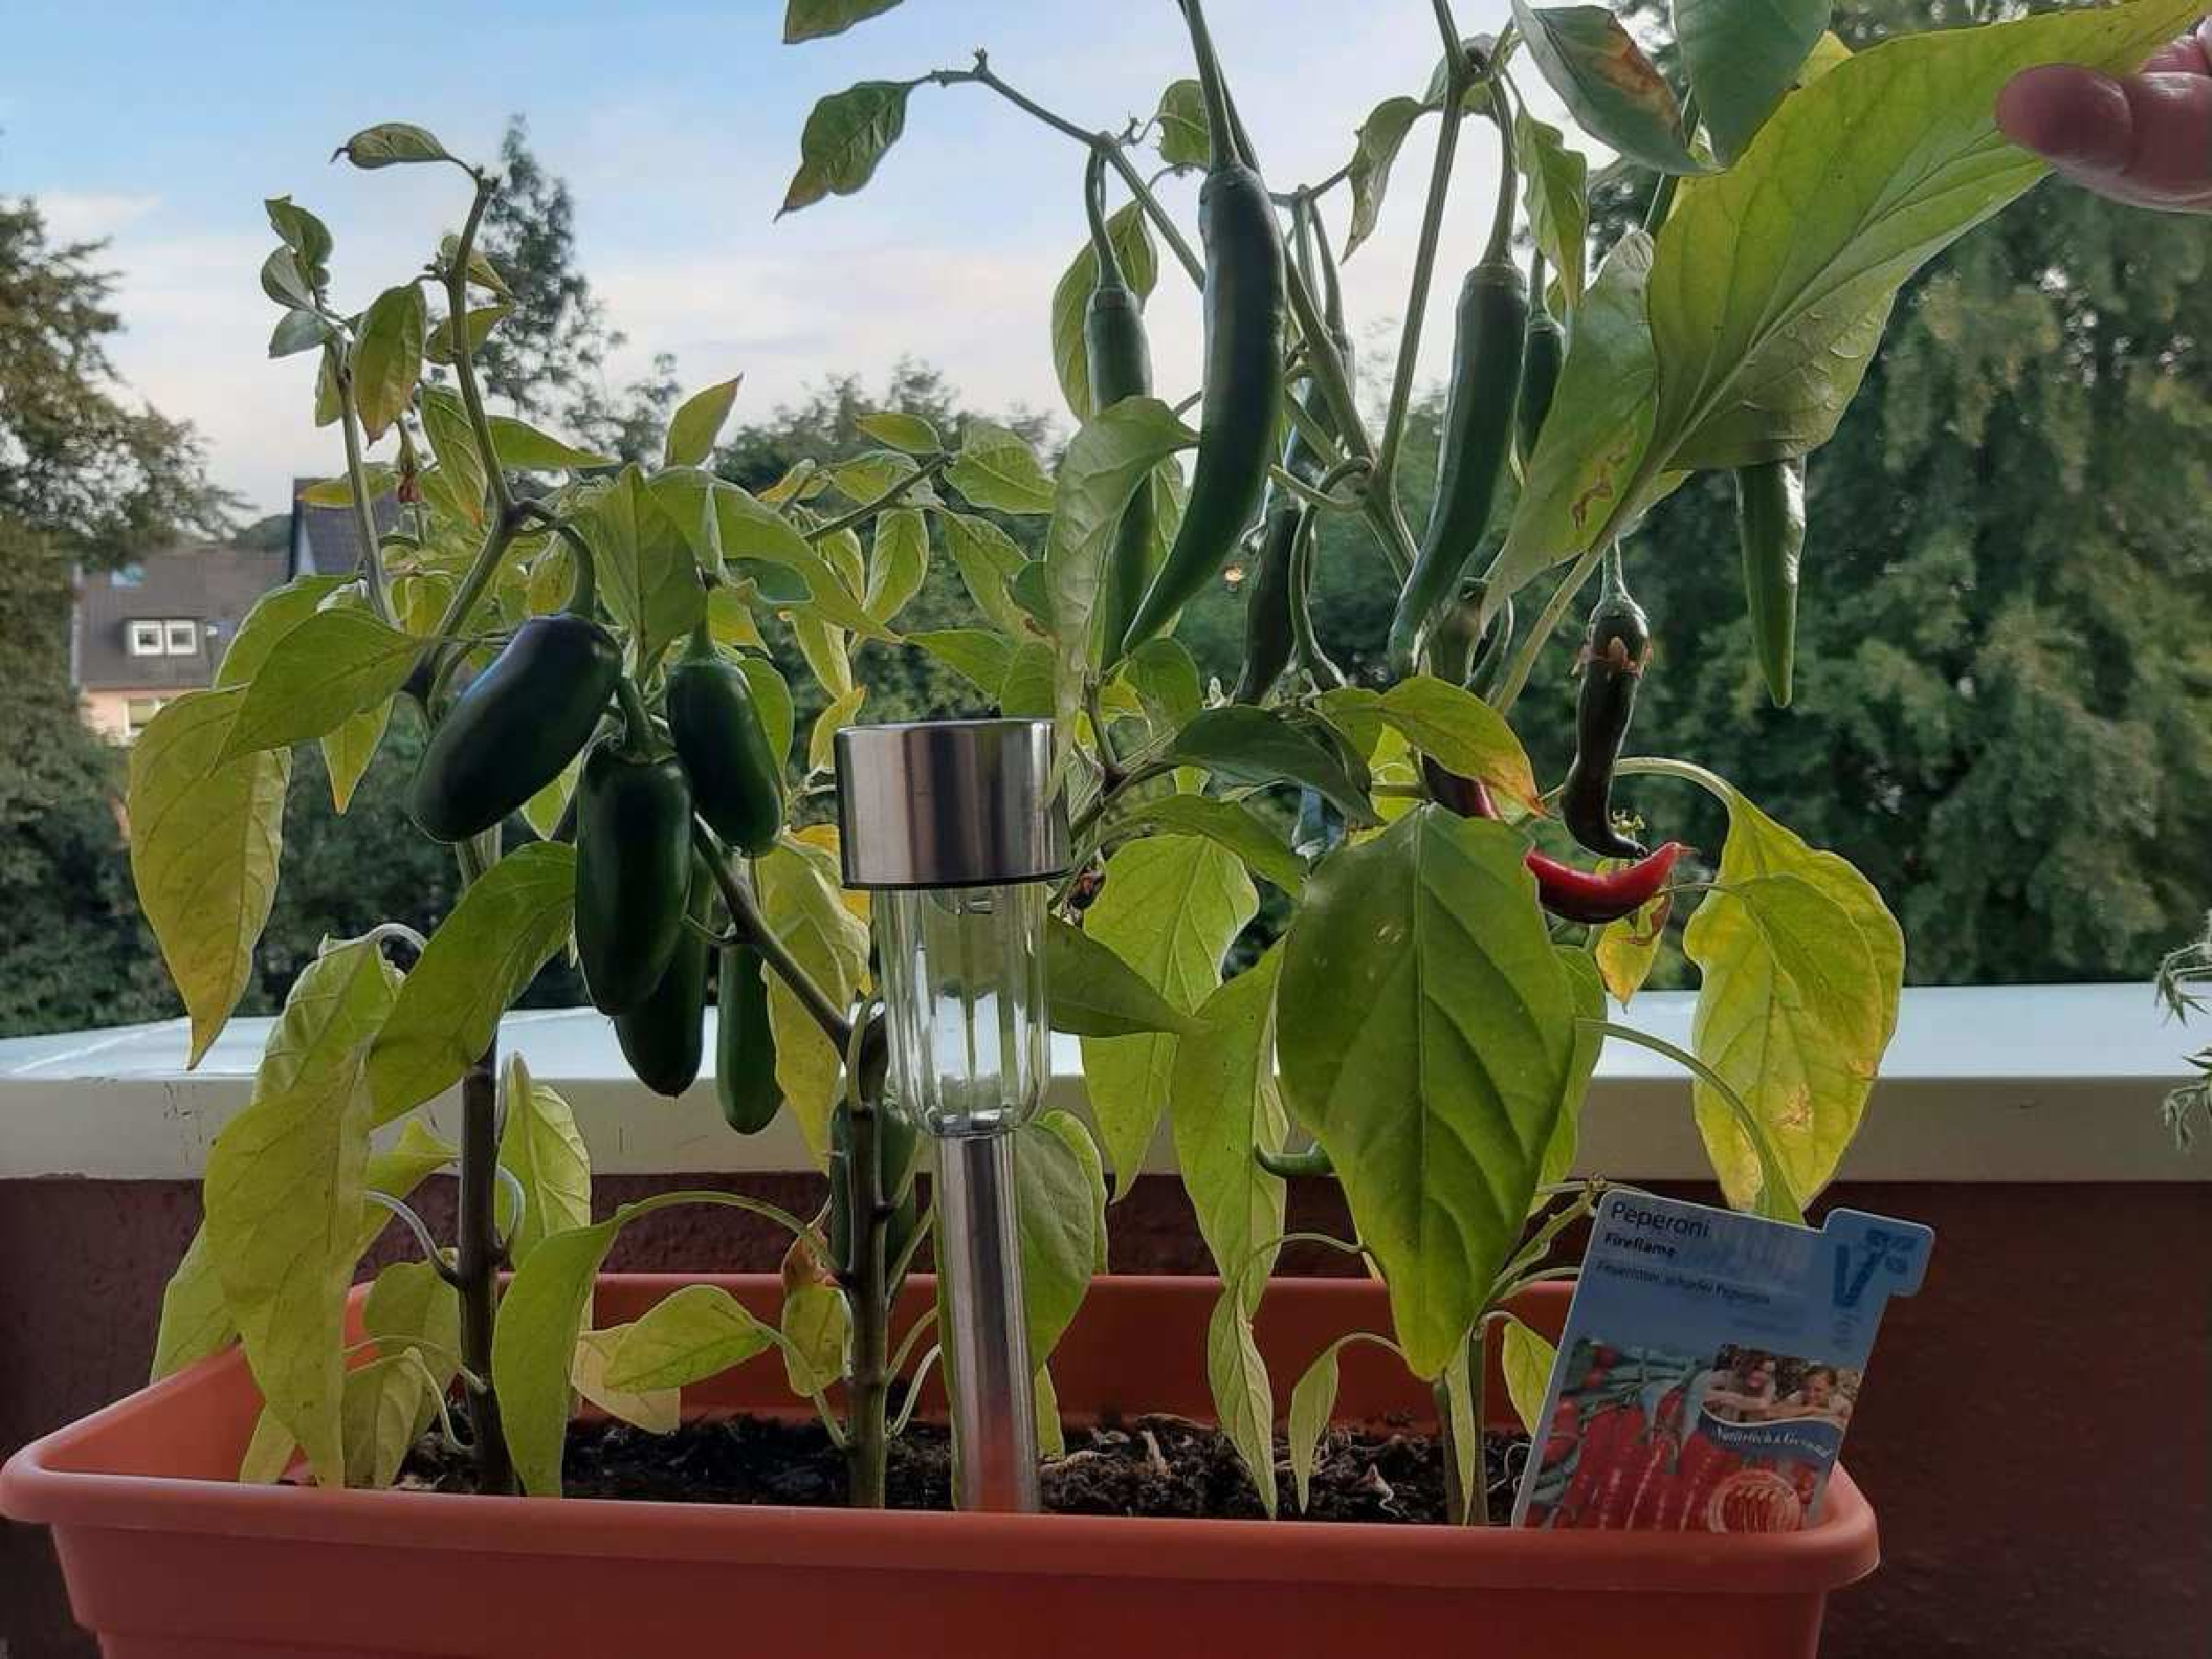
\includegraphics[width=0.6\textwidth]{images/Chili-1.pdf}
\caption{Abbildung-Bsp}
\label{fig:Abbildung-Bsp}%% anpassen
\end{figure}

\section{Tabelle}\label{tabelle}

Tabelle-Bsp vgl.~(\autoref{tab:Tabelle-Bsp}).

\begin{table}[!ht]% hier: !ht 
\centering 
	\caption{Tabelle-Bsp} \label{tab:Tabelle-Bsp}%% anpassen 
\begin{tabular}{@{}rll@{}}
\toprule
\textbf{Nr.} & \textbf{Begriffe} & \textbf{Erklärung}\\
\midrule
1 & a1 & a2\\
2 & b1 & b2\\
3 & c1 & c2\\
4 & a1 & a2\\
\bottomrule
\end{tabular} 
\end{table}

\section{Mathe}\label{mathe}

$[ V ] = [ \Omega ] \cdot [ A ]$ o. $U = R \cdot I$ o.
$R = \frac{U}{I}$

$800~cm$

$100^\circ\text{C} \, 5~\Omega$

\textbf{Matheumgebung:}

\begin{align*}
    \sum_{i=1}^5 a_i = a_1 + a_2 + a_3 + a_4 + a_5
\end{align*}

\section{Texthervorhebung}\label{texthervorhebung}

\textbf{Fett} oder \emph{Kursiv}

\section{Code}\label{code}

HalloWelt vgl.~(\autoref{code:HalloWelt}).

\lstset{language=C}% C, TeX, Bash, Python 
\begin{lstlisting}[
	caption={HalloWelt}, label={code:HalloWelt}%% anpassen
]
// hallowelt.c
#include <stdio.h>
int main(void) {
    printf("Hallo Welt!\n");
    return 0;
}
\end{lstlisting}

\section{Links}\label{links}

\url{https://google.de} oder \href{https://google.de}{Google}

Fussnote \footnote{\url{https://bw-ju.de/}}

\section{Absätze}\label{absaetze}

Dies hier ist ein Blindtext zum Testen von Textausgaben. Wer diesen Text
liest, ist selbst schuld. Der Text gibt lediglich den Grauwert der
Schrift an. Ist das wirklich so? Ist es gleichgültig, ob ich schreibe:
>>Dies ist ein Blindtext<< oder >>Huardest gefburn<<? Kjift -
mitnichten! Ein Blindtext bietet mir wichtige Informationen. An ihm
messe ich die Lesbarkeit einer Schrift, ihre Anmutung, wie harmonisch
die Figuren zueinander stehen und prüfe, wie breit oder schmal sie
läuft. Ein Blindtext sollte möglichst viele verschiedene Buchstaben
enthalten und in der Originalsprache gesetzt sein. Er muss keinen Sinn
ergeben, sollte aber lesbar sein.

Fremdsprachige Texte wie >>Lorem ipsum<< dienen nicht dem eigentlichen
Zweck, da sie eine falsche Anmutung vermitteln.

		%
		%-------------------------------------------------

	%\printindex% Index (Register)
	% Bibliographie
	%\phantomsection\addcontentsline{toc}{section}{Literatur}
	\printbibliography% Literaturverzeichnis
\end{document}
